%%%%%%%%%%%%%%%%%%%%%%%%%%%%%%%%%%%%%%%%%%%%%%%%%%%%%%%%%%%%%%%
% ACL 2027 (ACL Rolling Review) anonymous submission, built on the official
% ACL style files (acl.sty / acl_natbib.bst from github.com/acl-org/acl-style-files).
% Change "review" to "final" for the camera-ready version.
%%%%%%%%%%%%%%%%%%%%%%%%%%%%%%%%%%%%%%%%%%%%%%%%%%%%%%%%%%%%%%%
\documentclass[11pt]{article}
\usepackage[review]{acl}

% Standard package includes (from the ACL template)
\usepackage{times}
\usepackage{latexsym}
\usepackage[T1]{fontenc}
\usepackage[utf8]{inputenc}
\usepackage{microtype}
\usepackage{inconsolata}
\usepackage{graphicx}
\usepackage{adjustbox} % shrink over-wide floats to the column
\usepackage{xurl}      % allow line breaks anywhere in long reference URLs
\usepackage[normalem]{ulem} % \uline in Figure 1

% Algorithms (used by Algorithm 1)
\usepackage{algorithm}
\usepackage{algorithmic}

% Better-looking tables
\usepackage{booktabs}

% Vector figures
\usepackage{tikz}
\usetikzlibrary{arrows.meta,positioning,calc}

%%%%%%%%%%%%%%%%%%%%%%%%%%%%%%%%%%%%%%%%%%%%%%%%%%%%%%%%%%%%%%%
% Project-specific packages/macros
%%%%%%%%%%%%%%%%%%%%%%%%%%%%%%%%%%%%%%%%%%%%%%%%%%%%%%%%%%%%%%%
\usepackage{amsmath}
\usepackage{amssymb}
\usepackage{amsthm}
\usepackage{threeparttable}
\usepackage{xspace}
\usepackage{pifont}
\usepackage{enumitem}
\usepackage{textcomp}

\newtheorem{example}{Example}
\newtheorem{theorem}{Theorem}
\newtheorem{proposition}{Proposition}

\DeclareMathOperator{\E}{\mathbb{E}}
\DeclareMathOperator{\Var}{\mathrm{Var}}
\newcommand{\Xsafe}{\mathcal{X}_{\mathrm{safe}}}
\newcommand{\given}{\;\vert\;}
\newcommand{\cmark}{\ding{51}} % check mark (tables)
\newcommand{\xmark}{\ding{55}} % cross mark (tables)

% Each .bib entry carries note={\refurl{<url>}}. ACL permits hyperref, so the
% reference URL is printed as a clickable link. The bst emits
% `\newblock \refurl{URL}.', so the trailing period is kept.
\newcommand{\refurl}[1]{\url{#1}}

%%%%%%%%%%%%%%%%%%%%%%%%%%%% document %%%%%%%%%%%%%%%%%%%%%%%%%%%%
\title{SemantOS: Safe and Explainable Kernel Tuning via Semantic Reasoning and Guardrailed LLMs}
\author{Anonymous Submission}
\affiliations{Research revision --- prototype and evaluation protocol}


\begin{document}
\maketitle

\begin{abstract}
Language models increasingly recommend actions and justify them with citations to evidence in the prompt. Such a rationale makes three promises: the action is good, its claims about the evidence are true, and the decision rests on what is cited. Evaluations rarely test all three, or compare against what the evidence alone would recommend. Our audit protocol gives an equally informed non-LLM selector the same frozen evidence, ablates and deletes evidence, verifies every quantitative claim in an explanation against it, and scores decisions on independently labeled held-out outcomes. We apply it to configuration advice on real Linux kernel interventions with \sysname, a testbed separating evidence, proposals and enforcement, and ten LLMs from 7B to frontier scale. The promises come apart. Evidence is necessary: without it, nine models mostly choose worse. It is also sufficient: with it, nine reproduce a table-lookup selector and none improves on it. Citations are valid but one-sided: 252 of 260 cited runs belong to the chosen configuration. Explanations are cited but not correct: 41 of 97 audited claims misstate the evidence, mostly alongside a correct decision, and deletion reveals citation-specific reliance for only one model. Prompts, responses, annotations, code and logs are provided as supplementary material.
\end{abstract}

\section{Introduction}
\label{sec:introduction}
Kernel tuning requires choosing configurations whose effects depend on workload, hardware and the current operating state, and a setting that improves one metric can worsen another. Learned tuners have long been applied to databases and data-processing systems~\cite{VanAken2017OtterTune,Zhang2019CDBTune,Herodotou2020Survey}, and language models now read manuals, propose complete configurations, or search kernel build options~\cite{Trummer2022DBBERT,Lao2024GPTuner,Giannakouris2025LambdaTune,Chen2024AutoOS,Lin2025TuneAgent}. Two questions are nevertheless hard to answer from existing evaluations. Does a language model add value beyond the information already present in its knowledge base (KB) when a conventional optimizer receives the same inputs? And when a proposal is applied, is the risk of harm measured by an outcome that does not depend on the enforcement mechanism itself?

SemantOS is designed to make both questions testable. It separates three responsibilities: evidence acquisition, candidate generation and enforcement. A typed graph and retrieved traces expose the available evidence; a reasoner proposes a multi-knob bundle; and a runtime checks the complete bundle and decides whether to veto it or enter a staged rollout. Because the evidence is explicit, the same evidence can be handed to a non-LLM optimizer; because enforcement is independent, its errors can be counted against labels defined from raw observations.

\paragraph{Contributions.}
(i)~A bundle-level control contract, with a dry-run REST implementation and a separate actuator that applies, verifies and restores per-thread kernel settings (see SemantOS Design). (ii)~An expected-cost identity for gated acceptance and a restricted rank gate, stated with the conditioning and assumptions under which they hold (see Probability Statements for Gated Acceptance). (iii)~A role-separated evaluation protocol that freezes selections and thresholds before test data are opened and reports every denominator, applied to real Linux interventions (see Measurements and Evaluation Protocol). The measured results are deliberately reported even where unfavorable: informed non-LLM selectors yield no gain over the default, four open-weight LLMs do no better, and the frozen gate misses more unsafe runs than its nominal level under a period shift.

\paragraph{Scope.}
The REST runtime never writes kernel settings, and the actuator changes only an owned child thread. We therefore make no deployment-efficacy, production-safety or LLM-superiority claim; the Evaluation Protocol section lists the matched comparisons that such claims require.

\section{Related Work}
\label{sec:background}
\paragraph{Attribution in grounded generation.}
Retrieval-augmented generation conditions outputs on retrieved documents~\cite{Lewis2020RAG}, and a line of work asks whether the resulting text is supported by what it cites. AIS defines attribution to identified sources~\cite{Rashkin2023AIS}; Attributed QA and ALCE benchmark answers and citations for support~\cite{Bohnet2022AttributedQA,Gao2023ALCE}; RARR retrofits attribution by revising unsupported text~\cite{Gao2023RARR}; and an audit of generative search engines found many statements not fully supported by the sources they cite~\cite{Liu2023Verifiability}. FActScore decomposes long outputs into atomic facts checked against a knowledge source~\cite{Min2023FActScore}. We share the claim-level view but check claims exactly against a small, structured evidence set supplied in the prompt, and we pair explanation checks with a decision-level baseline that receives the same evidence.

\paragraph{Accuracy of generation from data.}
Data-to-text generation has long documented factual errors in text produced from tables and records~\cite{Wiseman2017DataToDocument}. \citet{Thomson2020GoldStandard} annotate every factual error in generated basketball summaries against the source data, with categories that include incorrect numbers, names and words, and summarization work separates intrinsic from extrinsic hallucination~\cite{Maynez2020Faithfulness,Ji2023HallucinationSurvey}. Table-based fact verification and logical table-to-text generation show that statements requiring comparison, superlatives or aggregation over a table are hard both to verify and to generate faithfully~\cite{Chen2020TabFact,Chen2020LogicNLG}. Our taxonomy follows this tradition: the dominant errors we observe are exactly such superlative, range and quantifier claims over a numeric table, now made by instruction-tuned LLMs in free-text rationales.

\paragraph{How models use supplied context.}
When supplied context conflicts with parametric knowledge, models may ignore it~\cite{Longpre2021KnowledgeConflicts} or accept coherent counter-evidence while favoring their priors~\cite{Xie2024ChameleonSloth}; irrelevant context distracts them~\cite{Shi2023Distracted}, and information in the middle of long contexts is used less~\cite{Liu2024LostMiddle}. Our evidence ablation measures the complementary case in which the context is decisive and the parametric prior is misleading: without evidence, models invent meanings for opaque configuration names.

\paragraph{Faithfulness of explanations.}
Faithfulness must be evaluated separately from plausibility~\cite{Jacovi2020Faithfulness}. ERASER measures the comprehensiveness and sufficiency of rationales by removing them~\cite{DeYoung2020ERASER}; counterfactual and reconstruction tests probe natural-language explanations~\cite{Atanasova2023FaithfulnessTests}; and chain-of-thought explanations can omit the factors that drive a prediction~\cite{Turpin2023Unfaithful} or be tested by intervening on the reasoning~\cite{Lanham2023CoTFaithfulness}. Self-explanation faithfulness varies across models and tasks~\cite{Madsen2024SelfExplanations}, and many such tests measure output-level self-consistency rather than faithfulness to the model's internals~\cite{Parcalabescu2024SelfConsistency}. ContextCite attributes generations to context by ablation~\cite{CohenWang2024ContextCite}. Our matched deletion is an ERASER-style comprehensiveness test with a same-kind uncited control; in the terms of \citet{Parcalabescu2024SelfConsistency} it measures whether the decision is sensitive to what is cited, not whether the explanation mirrors internal computation.

\paragraph{LLMs as optimizers and configuration advisors.}
LLMs can optimize by proposing candidates from past evaluations~\cite{Yang2024OPRO}. DB-BERT mines tuning hints from manuals~\cite{Trummer2022DBBERT}, GPTuner uses LLM-extracted knowledge to prune a Bayesian-optimization search~\cite{Lao2024GPTuner}, and $\lambda$-Tune generates complete configurations~\cite{Giannakouris2025LambdaTune}; AutoOS and TuneAgent tune Linux kernel build options with LLM agents~\cite{Chen2024AutoOS,Lin2025TuneAgent}. Classical tuners use Gaussian processes, reinforcement learning or black-box optimization~\cite{VanAken2017OtterTune,Zhang2019CDBTune,Herodotou2020Survey,Snoek2012BO,Golovin2017Vizier,Lee2022STUN}. These works report end-to-end gains; we instead ask what the language model adds over a selector given the same evidence, and whether its stated reasons are correct. We do not compare head to head with these systems.

\paragraph{Uncertainty and selective prediction.}
Self-consistency aggregates sampled outputs~\cite{Wang2023SelfConsistency}; LLMs can partly predict their own correctness~\cite{Kadavath2022Know}, verbalized confidence can be better calibrated than token probabilities for RLHF models~\cite{Tian2023JustAsk} yet remains overconfident~\cite{Xiong2024ExpressUncertainty}, and semantic entropy measures uncertainty over meanings~\cite{Kuhn2023SemanticUncertainty}. Selective classification abstains to meet a target risk~\cite{Geifman2017Selective}, and conformal methods give distribution-free guarantees for language-model outputs~\cite{Quach2024ConformalLM}, their factuality~\cite{Mohri2024ConformalFactuality} and monotone losses~\cite{Angelopoulos2024CRC}, with extensions for non-exchangeable or drifting data~\cite{Farinhas2024NCRC,Barber2023Beyond,Gibbs2021ACI}. None implies that a window reset after a detected change~\cite{Bifet2007ADWIN} restores a fixed risk level. Our rank gate is a restricted class-conditional instance of this family, and we report where its assumptions fail.

\paragraph{Evaluation methodology.}
Random or standard splits can overestimate performance under realistic shift~\cite{Gorman2019StandardSplits,Sogaard2021RandomSplits}, and comparisons are fair only when budgets are reported and matched~\cite{Dodge2019ShowYourWork}. Our protocol applies these principles to LLM advisors: evidence, calibration and test roles come from disjoint operating conditions frozen in advance, and every non-LLM baseline receives the same evidence and an explicit evaluation budget.

\section{Testbed: \sysname}
\label{sec:testbed}
\sysname is an evidence-grounded generation pipeline for system configuration that we use as an instrument (Figure~\ref{fig:runtime-path}). Four properties matter for the audit. The evidence is \emph{addressable} (every citation resolves to one item), \emph{portable} (a non-LLM selector can receive the same object) and \emph{editable} (kinds or items can be removed), and enforcement is \emph{independent} of generation, so its errors can be counted against labels the generator never sees.

\paragraph{Evidence as a structured context.}
The store holds typed items, each with a stable ID, a kind and a provenance record: summary tables, individual measurement traces, and edges of a knob-interaction graph. The graph is a small knowledge representation with a strict admission rule: for a lower-is-better loss $L$ and baseline values $a_0,b_0$, an edge requires the contrast $I_{ab}=L(a,b)-L(a,b_0)-L(a_0,b)+L(a_0,b_0)$ from independently measured configurations, with a bootstrap interval over runs that excludes zero, and records its scope, values, measurement IDs and interval. Edges describe empirical interactions, not causal couplings (Appendix~\ref{app:testbed}). For the audit, the evidence is frozen and serialized as a JSON list that is identical for every advisor.

\paragraph{Generation.}
The reasoner retrieves typed neighbors and lexically matched trace text~\cite{Lewis2020RAG} and asks a model for a complete proposal, a set of knob values, with cited item IDs and an explanation. In deployment it draws $k=3$ samples~\cite{Wang2023SelfConsistency} and returns a modal complete proposal actually present in a response, rather than splicing per-knob winners into an unseen combination, scores each member by sample disagreement $u$ (a heuristic, not a calibrated probability; Appendix~\ref{app:testbed}), and abstains when no model responds or the context budget would force evidence to be truncated. The audit in \S\ref{sec:protocol} calls each model directly on the frozen evidence, one response per seed, so that decisions, citations and explanations can be compared across models without the aggregation step.

\begin{figure}[t]
\centering
\begin{adjustbox}{max width=\columnwidth}
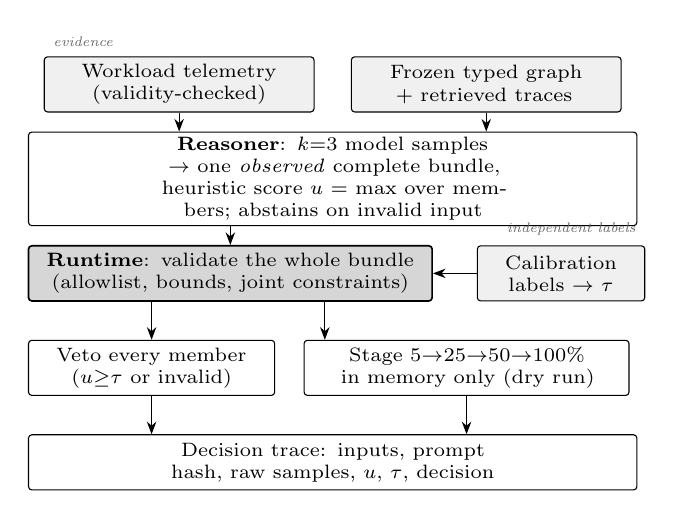
\begin{tikzpicture}[font=\scriptsize, >={Stealth[length=1.6mm]}, x=1mm, y=1mm,
  box/.style={draw, rounded corners=1.2pt, align=center, inner sep=1.8pt, minimum height=7mm},
  ev/.style={box, fill=black!6}, en/.style={box, fill=black!16, line width=0.6pt},
  tag/.style={font=\tiny\itshape, text=black!60}]
\node[ev, text width=33mm] (tel) at (-19.5,0) {Workload telemetry\\(validity-checked)};
\node[ev, text width=33mm] (kb)  at (19.5,0)  {Frozen typed graph\\+ retrieved traces};
\node[box, text width=76mm] (rsn) at (0,-12) {\textbf{Reasoner}: $k{=}3$ model samples $\rightarrow$ one \emph{observed} complete bundle,\\heuristic score $u$ = max over members; abstains on invalid input};
\node[en, text width=50mm] (val) at (-13,-24) {\textbf{Runtime}: validate the whole bundle\\(allowlist, bounds, joint constraints)};
\node[ev, text width=20mm] (cal) at (29,-24) {Calibration\\labels $\rightarrow$ $\tau$};
\node[box, text width=30mm] (veto)  at (-23,-36) {Veto every member\\($u{\ge}\tau$ or invalid)};
\node[box, text width=40mm] (stage) at (17,-36) {Stage $5{\to}25{\to}50{\to}100\%$\\in memory only (dry run)};
\node[box, text width=76mm] (trace) at (0,-48) {Decision trace: inputs, prompt hash, raw samples, $u$, $\tau$, decision};
\draw[->] (tel) -- (tel |- rsn.north);
\draw[->] (kb) -- (kb |- rsn.north);
\draw[->] (rsn.south -| val) -- (val.north);
\draw[->] (cal) -- (val);
\draw[->] (val.south -| veto) -- (veto.north);
\draw[->] (val.south) ++(12,0) -- (stage.north -| {$(val.south)+(12,0)$});
\draw[->] (veto) -- (veto |- trace.north);
\draw[->] (stage) -- (stage |- trace.north);
\node[tag, anchor=south west] at (tel.north west) {evidence};
\node[tag, anchor=south east] at (cal.north east) {independent labels};
\end{tikzpicture}
\end{adjustbox}
\caption{\sysname decision path. Evidence, generation and enforcement are separate components: the frozen evidence object can be given to a non-LLM selector, ablated or partially deleted, citations can be resolved against its item IDs, and gate errors can be counted against independently defined labels. The REST runtime is a dry run; a separate per-thread actuator applies, verifies and restores timer slack and affinity in owned child processes.}
\label{fig:runtime-path}
\end{figure}

\paragraph{Enforcement.}
The runtime treats a proposal as a unit: it validates every member (allowlisted knobs, bounds, joint constraints, no duplicates) and, if any member score satisfies $u\ge\tau$, vetoes all of them; otherwise the proposal enters a staged rollout. The REST runtime is a dry run that never writes kernel settings (Appendix~\ref{app:testbed}). The threshold $\tau$ comes from a rank gate, a selective-prediction rule~\cite{Geifman2017Selective} calibrated on unsafe examples only. Let $Y=1$ denote an unsafe outcome defined from raw observations, never from whether a veto or rollback occurred.
\label{subsec:theorem}
\begin{proposition}[Restricted rank gate]\label{prop:recal}
Fix a score function before calibration. Suppose $n$ unsafe calibration scores and the next unsafe test score are jointly exchangeable. Set $j=\lfloor\alpha(n+1)\rfloor$ for $0<\alpha<1$. If $j=0$, veto all; otherwise let $\tau$ be the $j$th smallest unsafe calibration score and accept only when $u<\tau$. Then the unsafe-class acceptance probability, marginal over calibration and test scores, is at most $j/(n+1)\le\alpha$.
\end{proposition}
\noindent\emph{Proof.} By exchangeability the test score's rank among the $n+1$ scores is uniform; it falls below the $j$th calibration score only in the first $j$ ranks, and ties only reduce this.\hfill$\square$

The bound controls misses among unsafe actions, $\Pr(A=1\mid Y=1)$, not the unsafe fraction among accepted actions; a cost-selected threshold is capped at the rank threshold, and no unsafe calibration example implies veto-all. The gate accepts any fixed score; \S\ref{subsec:gate} evaluates it with a measured risk score rather than $u$. An expected-cost identity, a discussion of drift and the bounded per-thread actuator used in \S\ref{subsec:gate} are in Appendix~\ref{app:testbed}.

\section{Audit Protocol}
\label{sec:protocol}
\label{sec:evaluation}
\paragraph{Task.}
An advisor selects one of four per-thread configurations: timer slack of 50\,$\mu$s or 1\,ms (set by \texttt{PR\_SET\_TIMERSLACK}) crossed with affinity to all four CPUs or to CPU~0, named \texttt{s50000\_aall}, \texttt{s50000\_aone}, \texttt{s1000000\_aall} and \texttt{s1000000\_aone}. The objective is the 95th-percentile (P95) lateness of periodic wake-ups against absolute monotonic-clock targets, and \texttt{s50000\_aall} is the explicit control. Every measurement runs in a fresh owned child process that checks kernel readback, on an Intel Core i5-3570 host (four logical CPUs, Linux 6.17); no host-wide setting is changed.

\paragraph{Role separation.}
The plan was saved before acquisition. Training, retrieval, calibration and test use wake-up periods of 2, 3, 4 and $\{5,8\}$\,ms. Each period has ten randomized blocks of the four configurations, with five warm-ups and 40 recorded events per child: 200 processes and 8,000 events. Roles are period-disjoint but share one workload family and host. Selections and thresholds are frozen, with hashes, before calibration and test data are opened, and a validator rejects role overlap or unknown lineage.

\paragraph{Frozen evidence.}
The evidence given to every advisor contains three kinds of items: the training table (mean training-run P95 per configuration), an interaction-graph item (the training contrast, $-18.6\,\mu$s, whose prespecified bootstrap interval includes zero, so the graph has no edge), and 40 retrieval items, each a single retrieval run's configuration, period and P95. Test outcomes never enter a prompt.

\paragraph{Equally informed baselines.}
The table selector minimizes mean training P95; a saturated two-factor model of the same four means adds no information. Both use the same 40 training runs as the LLMs and no online trials. Unchanged-control and seeded uniform-random selectors are references. Matched-budget random search, $\epsilon$-greedy Q-learning ($\epsilon=0.1$), UCB1~\cite{Auer2002UCB} and Gaussian-process expected-improvement BO~\cite{Snoek2012BO} each evaluate $B\in\{4,8,16,40\}$ training runs, starting with one per configuration and drawing recorded runs with replacement; $B=40$ matches the table selector.

\paragraph{LLM conditions.}
Qwen2.5 7B and 14B~\cite{Qwen2024Qwen25}, Llama-3.1-8B~\cite{Grattafiori2024Llama3} and Phi-4~\cite{Abdin2024Phi4} run locally as hashed 4-bit GGUF files in llama.cpp. Llama-3.3-70B, Qwen3-235B-A22B~\cite{Yang2025Qwen3}, DeepSeek-V3.2~\cite{DeepSeek2025V32}, Nemotron-3-Ultra-550B~\cite{NVIDIA2026Nemotron3Ultra}, Gemini~3.8 Flash~\cite{Google2026Gemini38Flash} and Gemini~3.1 Pro preview~\cite{Google2026Gemini31Pro} run through OpenRouter; their weights cannot be hashed. All models receive the same system prompt, JSON evidence and schema (a configuration from the allowed list, at most six citations restricted to supplied IDs, and an explanation of at most 400 characters; Appendix~\ref{app:prompt}), with temperature~0 and five seeds. DeepSeek-V3.2's providers did not enforce the length limit in 14 of its 20 answers (up to 931 characters); these answers are kept and audited in full. Four input variants are compared: full evidence, no graph, no retrieval, and no evidence.

\paragraph{Reliance by matched deletion.}
Following the comprehensiveness test of ERASER~\cite{DeYoung2020ERASER}, for each seed we delete the evidence items cited in the full-context answer and, separately, the same number of uncited items of the same kinds. A decision that changes only when cited items are deleted indicates citation-specific reliance. A seed is non-estimable when no same-kind uncited control exists; in particular, the training table is the only table item, so an answer citing it has no matched control.

\paragraph{Claim verification.}
Following error-annotation practice in data-to-text evaluation~\cite{Thomson2020GoldStandard}, every quantitative or comparative claim in each distinct explanation is checked against the supplied prompt evidence and labeled \emph{correct}, \emph{overstated}, \emph{wrong} (including partly wrong), \emph{wrong unit}, \emph{wrong attribution} (a value assigned to the wrong evidence source) or, for no-evidence prompts, \emph{unsupported prior}. A claim is \emph{misstated} if it is wrong, misattributed, overstated or in the wrong unit. A statement that a configuration is ``consistently'' or ``always'' lowest is labeled overstated, since the chosen configuration is lowest in 8 of 10 retrieval blocks. Local models returned byte-identical text across seeds, so each distinct explanation is audited once in every variant; hosted models varied across seeds and providers, so all distinct full-context explanations are audited. The labels were assigned by one annotator (an author) and are released per claim.

\paragraph{Outcomes and scoring.}
Each fixed choice is scored by paired offline replay on the measured test grid: the chosen configuration's run P95 in each block, and its paired change relative to the control in the same block, with a Student-$t$ interval across the ten blocks. A test run is \emph{unsafe} when more than 10\% of its 40 events exceed a predeclared 200\,$\mu$s deadline, a label computed from timing alone.

\section{Results}
\label{sec:results}
\label{subsec:followup}
We report the audit at four levels, from the decision to the text that justifies it: what models choose (\S\ref{subsec:decisions}), what they cite (\S\ref{subsec:citations}), what their explanations claim (\S\ref{subsec:claims}) and whether the cited evidence matters (\S\ref{subsec:reliance}). A final subsection evaluates the testbed's risk gate (\S\ref{subsec:gate}).

\subsection{Decisions: Evidence Is Necessary and Sufficient}
\label{subsec:decisions}
\begin{table}[t]
\centering\footnotesize\setlength{\tabcolsep}{2.5pt}
\caption{LLM decisions with evidence (full, no graph, no retrieval), without it, and after deleting cited or matched uncited evidence; superscripts count seeds; n/e: non-estimable; $^\dagger$hosted. Paired test P95 change versus control at 5 and 8\,ms (\%, 95\% half-width): ctrl 0; \protect50/1 $-145\pm125$ and $-180\pm156$; 1m/all $-599\pm188$ and $-631\pm179$; 1m/1 $-631\pm183$ and $-699\pm206$
\unskip.}
\label{tab:model-audit}
\begin{adjustbox}{max width=\columnwidth}
\begin{tabular}{@{}llccc@{}}
\toprule
Model & Context & Choice & 5\,ms & 8\,ms \\
\midrule
Qwen-7B & evidence & 50\,$\mu$s/all & 0 & 0 \\
 & none & 50\,$\mu$s/one & $-145\pm125$ & $-180\pm156$ \\
\addlinespace[2pt]
Llama-8B & all four & 50\,$\mu$s/one & $-145\pm125$ & $-180\pm156$ \\
 & del.\ cited & 1\,ms/all & $-599\pm188$ & $-631\pm179$ \\
 & del.\ unc. & 50\,$\mu$s/all & 0 & 0 \\
\addlinespace[2pt]
Qwen-14B & evidence & 50\,$\mu$s/all & 0 & 0 \\
 & none & 50\,$\mu$s/one & $-145\pm125$ & $-180\pm156$ \\
\addlinespace[2pt]
Phi-4 & evid., del.\ unc. & 50\,$\mu$s/all & 0 & 0 \\
 & none & 1\,ms/one & $-631\pm183$ & $-699\pm206$ \\
 & del.\ cited & 50\,$\mu$s/one & $-145\pm125$ & $-180\pm156$ \\
\bottomrule
\end{tabular}

\end{adjustbox}
\end{table}

The table selector and its saturated-model equivalent choose the control, which is also best on the test grid, so any other choice is a loss; control test P95 is $179.7\pm102.0$ and $155.7\pm64.4\,\mu$s at 5 and 8\,ms (95\% half-widths across ten blocks). Matched-budget random search, Q-learning, UCB1 and BO converge on it as well, choosing it in 98--99\% of 1,000 seeds at $B=40$ (Appendix~\ref{app:measurements}).

Table~\ref{tab:model-audit} gives each model's choice under every input condition. With evidence, nine of ten models choose the control in all three evidence variants, exactly as table lookup does; Llama-3.1-8B instead picks \texttt{s50000\_aone}, which is worse on replay ($-145\pm125\%$ and $-180\pm156\%$). Removing the graph item changes no choice, and removing the retrieval runs changes none either: the training table alone suffices. Without evidence, every model except Nemotron, which declares the default, chooses a worse setting in at least four of five seeds, usually single-CPU affinity with 50\,$\mu$s slack (six models) or with 1\,ms slack (three). The evidence is therefore necessary; in this task it is also sufficient, since no model improves on the selector that simply reads it. 249 of 250 calls returned schema-valid output.

\subsection{Citations: Valid, One-Sided and Front-Loaded}
\label{subsec:citations}
Every citation refers to a supplied item, since the schema permits nothing else, but what models choose to cite is far from a balanced account of the evidence. Across the 50 full-context answers, 285 citations comprise 25 of the training table, none of the interaction-graph item, and 260 of individual retrieval runs. Of these 260, 252 are runs of the configuration the model chose; only Gemini~3.1 Pro ever cites a run of a competing configuration. The cited evidence is thus confirmatory: no answer from the other nine models cites a run of a competing configuration, although \texttt{s50000\_aone} beats the control in two of ten retrieval blocks.

Citations also favor the start of the evidence list. Retrieval runs appear in block order, and 209 of the 260 retrieval citations fall in the first five of ten blocks. Seven models cite exactly a prefix of the blocks, typically blocks 0--4 or 0--5 of the chosen configuration, and so never cite that configuration's lowest run (block~7 for the control, block~8 for \texttt{s50000\_aone}). The six-citation cap in the schema makes a prefix convenient, but it does not explain why the prefix is chosen over the most informative runs; the pattern is consistent with the position effects reported for long contexts~\cite{Liu2024LostMiddle}.

\subsection{Explanations: Cited but Not Correct}
\label{subsec:claims}
\begin{table}[t]
\centering\footnotesize\setlength{\tabcolsep}{2.5pt}
\caption{Verification of quantitative and comparative claims in explanations against the supplied evidence (AI-drafted labels, verified by an author). Corr.: correct; Over.: overstated; Wrong: wrong or partly wrong value; Unit/Src: wrong unit or evidence source; Prior: unsupported prior without evidence; Misst.: wrong, misattributed, overstated or wrong unit. Generated by \texttt{claim\_taxonomy.py}.}
\label{tab:claims}
\begin{adjustbox}{max width=\columnwidth}
\begin{tabular}{@{}lrrrrrrr@{}}
\toprule
Model & $n$ & Corr. & Over. & Wrong & Unit/Src & Prior & Misst. \\
\midrule
Qwen-7B & 5 & 1 & 1 & 1 & 1 & 1 & 3 \\
Llama-8B & 7 & -- & -- & 6 & -- & 1 & 5 \\
Qwen-14B & 6 & 1 & 1 & -- & 3 & 1 & 4 \\
Phi-4 & 10 & 5 & 3 & 1 & -- & 1 & 4 \\
\textit{Local, all variants} & \textit{28} & \textit{7} & \textit{5} & \textit{8} & \textit{4} & \textit{4} & \textit{16} \\
\midrule
Llama-70B & 7 & 5 & -- & 2 & -- & -- & 2 \\
Qwen3-235B & 6 & 3 & 3 & -- & -- & -- & 3 \\
DeepSeek-V3.2 & 16 & 10 & 2 & 4 & -- & -- & 6 \\
Nemotron-550B & 23 & 13 & 5 & 5 & -- & -- & 10 \\
Gemini-Flash & 12 & 10 & 2 & -- & -- & -- & 2 \\
Gemini-Pro & 5 & 3 & 2 & -- & -- & -- & 2 \\
\textit{Hosted, full context} & \textit{69} & \textit{44} & \textit{14} & \textit{11} & \textit{--} & \textit{--} & \textit{25} \\
\bottomrule
\end{tabular}

\end{adjustbox}
\end{table}

\begin{table}[t]
\centering\footnotesize\setlength{\tabcolsep}{3pt}
\caption{Examples of misstated claims (paraphrased as audited) and the check against the supplied evidence; all latencies in $\mu$s.}
\label{tab:claim-examples}
\begin{tabular}{@{}p{0.25\columnwidth}p{0.36\columnwidth}p{0.33\columnwidth}@{}}
\toprule
Model, label & Claim & Evidence \\
\midrule
Gemini-Pro$^\dagger$, overstated & control ``consistently the lowest in retrieval runs'' & lowest in 8 of 10 blocks \\
Nemotron$^\dagger$, wrong & \texttt{s50000\_aone} ranges from 85.0 to 430.7 & maximum is 571.84 \\
DeepSeek$^\dagger$, wrong & control ``consistently lower than any'' \texttt{s50000\_aone} run & ranges overlap: 85.033 $<$ 183.217 \\
Qwen-7B, wrong source & training table gives control 126.36 & 126.36 is one retrieval run; training mean 132.94 \\
Qwen-14B, wrong unit & training table gives control 132.9413\,ms & evidence is in $\mu$s \\
Qwen-14B, prior & ``50000'' denotes a smaller dataset size & no evidence given; name is opaque \\
\bottomrule
\end{tabular}
\end{table}

The explanations are often wrong about what the cited items say (Table~\ref{tab:claims}): 16 of 28 audited claims from local models and 25 of 69 from hosted models are misstated. Errors fall into four recurring patterns (Table~\ref{tab:claim-examples}).

\emph{Overstated regularities.} Thirteen of the 19 overstatements assert that the chosen configuration is lowest ``consistently'' or in ``all'' retrieval runs, whereas it is lowest in 8 of 10 retrieval blocks; the other six claim ``significant'' differences that no test in the evidence supports. These claims are easier to make when, as above, the cited runs are all of one configuration.

\emph{Range and extremum errors.} All 11 wrong values from hosted models misreport a range, an extremum or a cross-configuration ordering. Nemotron repeatedly gives the \texttt{s50000\_aone} range as 85.0--430.7\,$\mu$s (its maximum is 571.84), and DeepSeek-V3.2 states that the control is ``consistently lower than any'' \texttt{s50000\_aone} run although the ranges overlap (Figure~\ref{fig:teaser}). Llama-3.1-8B reports 571.84\,$\mu$s, the \emph{maximum} of \texttt{s50000\_aone}, as the lowest P95, consistent with its wrong choice.

\emph{Source and unit confusion.} Qwen2.5-7B attributes the retrieval value 126.36 to the training table, whose mean is 132.94; Qwen2.5-14B reports the training mean 132.9413 in milliseconds in three explanations, although the evidence declares microseconds.

\emph{Invented semantics.} Without evidence, all four local models justify their choice by assigning meanings to opaque identifiers, for instance reading ``50000'' as a smaller dataset size or ``one'' as a more aggressive approach. The configuration names carry no such information.

These errors are largely decoupled from the decision: 35 of the 41 misstated claims accompany a choice of the control. Nor does variation in wording track variation in decisions: hosted models produced two to five distinct full-context explanations each while choosing the control in every seed. Valid citations thus establish provenance, and a correct decision can coexist with an incorrect account of the evidence that supports it.

\subsection{Reliance: Rarely Estimable, Rarely Specific}
\label{subsec:reliance}
Five models cite the training table in their full-context answers, so matched deletion is non-estimable for them. Among estimable models, only Phi-4 shows citation-specific reliance: deleting its six cited retrieval runs changes its choice in all five seeds while matched uncited deletion does not, but the new choice (\texttt{s50000\_aone}) contradicts the training table that remains in the prompt. Llama-3.1-8B changes its choice under both deletions, which indicates sensitivity to context rather than reliance on what it cites. Llama-3.3-70B, Qwen3 and Nemotron change under neither, which is consistent with the remaining evidence still favoring the control but uninformative about reliance.

\subsection{Enforcement: A Calibrated Gate under Shift}
\label{subsec:gate}
A test run is \emph{unsafe} when more than 10\% of its 40 events exceed a predeclared 200\,$\mu$s deadline, a label computed from timing alone. For the gate, the score is a configuration's training deadline-miss fraction, fixed before calibration on 4\,ms runs only; all three prespecified $\alpha\in\{.05,.10,.20\}$ yield $\tau=.9225$ because the unsafe-score order statistics are tied. Every candidate is executed in an isolated process, so accepted and vetoed candidates both have observed outcomes (Figure~\ref{fig:gate-replay} in Appendix~\ref{app:measurements}).

Unsafe acceptance is $5/25=20.0\%$ and $4/24=16.7\%$ among unsafe runs, above the nominal 5\% and 10\% levels; unsafe fractions among accepted runs are $5/20$ and $4/20$, and veto precision is $20/20$ in each period. As with LLM explanations, a nominally calibrated signal is only as good as the exchangeability it assumes, and a period shift is enough to break it. The bounded actuator restored both original settings in all 80 staged executions (Appendix~\ref{app:measurements}).

\section{Discussion}
\label{sec:discussion}
\paragraph{What the protocol shows.}
Each component isolates a different failure. The matched-information baseline separates what the evidence determines from what the model adds; here the answer is nothing, a result invisible to an evaluation that compares an LLM advisor only with the unchanged default or with a cold-start optimizer. Evidence ablation shows the models do read the evidence, since removing it degrades nine of ten. Claim verification shows that reading is not the same as reporting: explanations with valid citations misstate a third or more of their quantitative content. Deletion shows that citation lists are weak evidence of reliance, and that reliance can only be estimated when the evidence contains matched alternatives.

\paragraph{Recommendations.}
For evaluating evidence-grounded advisors we recommend (i) giving a non-LLM selector exactly the model's evidence and reporting both; (ii) verifying explanation claims against the supplied evidence, with special attention to quantifiers (``consistently'', ``all''), ranges and units, which account for most misstatements at every model size; (iii) designing evidence sets so that deletion controls exist; and (iv) labeling outcomes from raw observations rather than from the enforcement mechanism under test.

\paragraph{When could an LLM add value?}
Our task gives the evidence everything needed to decide. An LLM could add value when the evidence is incomplete and prior knowledge, for example from documentation, carries information the measurements lack. Testing this requires tasks where the default is not optimal and where the protocol's baseline receives the same documents, which we leave to future work.

\section{Conclusion}
\label{sec:conclusion}
A rationale that cites evidence promises a good decision, true claims about the evidence, and reliance on what it cites. We audited these promises separately for LLM configuration advice, holding the evidence fixed across LLM and non-LLM advisors, ablating and deleting it, verifying explanation claims against it, and scoring decisions on independently labeled held-out outcomes. The promises came apart. Ten LLMs needed the evidence to choose well but added nothing beyond a selector that reads it; 41 of 97 audited claims misstated evidence that was validly cited, mostly alongside a correct decision; and deletion showed citation-specific reliance for only one model.

For NLP evaluation, these results suggest three practices. First, citation validity and passage-level support are not enough: an explanation can cite exactly the right items and still misreport what they contain, so attribution should be checked at the level of individual claims. Second, the errors that data-to-text research documented for tables, namely wrong numbers, superlatives, ranges and overstated regularities, persist in the free-text rationales of instruction-tuned models of every size we tested, and deserve targeted checks. Third, the value of a language model in decision support should be measured against a baseline that receives the same evidence, and decision quality and rationale correctness should be reported separately.

Two extensions would strengthen these conclusions: tasks in which the evidence is incomplete and documentation-derived priors could genuinely help, and multi-annotator or automatic verification of claims, which the structured evidence makes feasible. The protocol and released data are intended to make both measurable.


% Unnumbered sections required/permitted by ACL; they do not count toward
% the page limit.
\section*{Limitations}
\label{sec:limitations}
\paragraph{Scope of the prototype.}
The REST runtime is a dry run: it never writes kernel settings, and the separate actuator changes only an owned child thread's timer slack and affinity. The artifact therefore demonstrates a decision contract, a bounded per-thread actuator, raw measurements and non-LLM selector replay, but not a deployed VM-sysctl bundle actuator, traffic isolation or a verified trained checkpoint. We make no deployment-efficacy, production-safety or LLM-superiority claim; Section~\ref{sec:protocol} and Appendix~\ref{app:testbed} list the matched comparisons and deployment requirements such claims require. The staged adapter is not wired into the REST VM-sysctl runtime and does not establish traffic isolation or recovery from irreversible effects. The reasoner awaits model samples synchronously, so we make no fast-path latency or resource-footprint claim; a nonblocking deployment would separate synchronous enforcement from asynchronous proposals and version the objective weights, policy, graph and calibration snapshots per decision. Logs are append-only files within a process, without tamper resistance. Prompting a model to obey graph edges does not enforce those edges; independent validation is required, and the current REST runtime enforces only its explicit example constraints.

\paragraph{Task and annotation.}
The audited task has four candidate configurations, its evidence determines the best choice, and the default is best on the test grid; the audit can therefore expose missing added value and misreported evidence, but it cannot show that an LLM adds value on harder tasks. Claim labels were assigned by a single annotator (an author) without an agreement study; the per-claim labels and checks are released so that they can be re-annotated. The claim sample is small (97 claims), local explanations were byte-identical across seeds, and five seeds under greedy decoding are not independent samples.

\paragraph{Evaluation breadth.}
All controlled measurements use one periodic workload family on one shared host, with roles separated by period rather than by workload family or hardware. Measured graph induction on the training sweep emits no edge. Selector, BO and RL comparisons replay recorded runs rather than executing closed loops, and control is best on the tested grid, so these comparisons can reveal only losses. Run-level intervals describe variability on a shared host and do not account for uncontrolled interference, warm-cache bias or correlated system state; exploratory intervals are unadjusted for multiple comparisons and temporal dependence, and the closed-loop local load does not characterize queueing under an externally fixed arrival rate. The model audit is retrospective and small, and hosted runs are not reproducible bit for bit. The available telemetry prototype contains scheduler and block-I/O demonstration proxies, including timestamp-derived buckets; those are not end-to-end request latencies and must not calibrate an empirical SLO claim. The local benchmarks record completion, failure and deadline data for their narrow tasks but do not substitute for web serving, TPC-C, Kafka/Spark, GPU inference or audio pipelines.

\paragraph{Risk statements.}
The rank gate's assumptions can fail under drift, selective labeling, or a score model updated using calibration data, and the observed miss rates under a period shift already exceed the nominal level. Because calibration and test periods differ, runs share a host, and the proposition is marginal under exchangeability, the gate replay neither verifies its deployment assumptions nor establishes recovery. A canary can suffer harm before detection, and rollback cannot undo every side effect. No no-worse-than-default, catastrophic-regression prevention, Pareto superiority or universal safety claim follows from the prototype. Valid citations in model explanations establish provenance, not faithful or correct reasoning. These limitations define concrete measurements and engineering prerequisites for the next evaluation.

\section{Ethical Considerations}
SemantOS follows least privilege: the recommender has no direct write authority,
and only the safety runtime may execute validated transactions under staged
rollout and rollback policy. The workload generators included in the artifact
are synthetic smoke tests and are explicitly excluded from empirical claims.
Future benchmark or human-subject results will be reported only with auditable
provenance, the applicable approval and consent process, and de-identified
records sufficient to reproduce the stated analysis.


\bibliography{reference-data}

\appendix
\section{SemantOS Testbed Details}
\label{app:testbed}
\paragraph{Design hypotheses.}
SemantOS is motivated by three hypotheses. First, a configuration's utility may depend on workload and hardware. Second, joint knob effects may be non-additive. Third, performance, failure probability and intervention cost may conflict. Each hypothesis requires measured interventions with explicit baselines.

For a loss $L$, define an interaction contrast from four independently measured configurations:
\[
 I_{ab}=L(a,b)-L(a,b_0)-L(a_0,b)+L(a_0,b_0).
\]
For lower-is-better loss, negative $I_{ab}$ indicates a beneficial non-additive interaction relative to the chosen baseline. A bootstrap interval must resample independent runs, not individual requests from a single run. The sign can change with workload, value range or kernel version, so an edge needs its scope, configuration values, measurement IDs and uncertainty interval. Such an edge describes an empirical interaction, not an unconditional causal coupling.

A \textsc{depends-on} edge requires a validated admissibility rule or measured range conditioning; it cannot be inferred solely from the sign of $I_{ab}$. The released seed graph is empty until edges pass this test. The principal question is whether a reasoner can use independently acquired evidence more effectively than an optimizer with the same inputs, after charging the cost of acquiring that evidence.

\paragraph{Bundle contract.}
A request contains a nonempty bundle identifier and a list of recommendations with \texttt{id}, \texttt{knob}, \texttt{proposed}, \texttt{uncertainty}, and optional rationale and provenance. Each request submits one bundle. Duplicate knobs, nonfinite scores, unsupported controls, and example-policy bound violations reject the entire request. Dirty-ratio changes must supply both values and satisfy the example policy that the background ratio is less than the foreground ratio. This is a declared policy, not proof that a configuration improves any workload. If any score satisfies $u\ge\tau$, all members are vetoed; otherwise all are staged together. A concurrent bundle receives a conflict response. Dry-run results return \texttt{applied=[]} and list simulated members separately.

\begin{algorithm}[t]
\caption{Implemented dry-run bundle path}
\label{alg:control-loop}
\begin{algorithmic}[1]
\REQUIRE Validated bundle $B$, fixed score function, calibration threshold $\tau$
\STATE Validate every member and joint constraints before changing state
\IF{another bundle is active}
  \STATE Return conflict
\ENDIF
\IF{$\max_{a\in B}u(a)\ge\tau$}
  \STATE Record veto for all members; return
\ENDIF
\STATE Stage the complete bundle in memory at 5\%
\FOR{requested stage in $\{25,50,100\}\%$}
  \STATE Advance the simulated bundle; record the transition
\ENDFOR
\STATE On cancellation, clear the complete simulated bundle
\STATE Never infer an unsafe/safe training label from simulated completion
\end{algorithmic}
\end{algorithm}

\paragraph{Deployment requirements.}
A real actuator must snapshot all old values, validate the full target configuration and available host interfaces, serialize updates, verify readback, and restore every old value on failure. Multiple sysctl writes are not a kernel transaction: partial exposure must be measured and cannot be described as atomic hardware state. Canary shares require separate hosts or an appropriate isolation mechanism; changing a host-global sysctl cannot isolate a fraction of requests on that host. Missing, stale or malformed end-to-end telemetry must stop promotion. These capabilities are requirements, not features demonstrated by the dry-run state machine.

\paragraph{One illustrative decision trace.}
Consider supplied context with example values 5 and 15 for the two dirty ratios, and retrieved evidence IDs $e_1,t_1$. Suppose all three model samples agree on this pair and $w=0$, giving $u=0.30$. If an independently obtained threshold is $\tau=0.25$, the whole bundle is vetoed; if $\tau=0.35$, it can enter the dry-run canary after joint validation. The audit record includes the values, scores, threshold and decision. These numbers illustrate the contract and are not a measured recommendation or calibrated operating point. The initial artifact threshold is zero until calibration data is explicitly supplied.

\paragraph{Expected cost of gated acceptance.}
Let $Y=1$ denote an independently defined unsafe outcome and $A=1$ acceptance. An outcome label is not defined by whether a rollback happened. For example, a benchmark can predeclare a request deadline, count observed failures or deadline exceedances, and define an action-level breach from these raw observations in a fixed window. Rejected actions have unknown counterfactual outcomes unless evaluated in an isolated experiment; they must not automatically be labeled safe or unsafe.

\begin{theorem}[Cost identity]\label{thm:pac-cost}
For costs $c_{\rm FN},c_{\rm FP},\lambda\ge0$, define
$C=c_{\rm FN}\mathbf{1}\{Y=1,A=1\}+c_{\rm FP}\mathbf{1}\{Y=0,A=0\}+\lambda D$,
where $D\ge0$ is measured exposure or SLO debt. Write $\pi=\Pr(Y=1)$,
$q=\Pr(A=1\mid Y=1)$ and $r=\Pr(A=0\mid Y=0)$. Then
\[
\mathbb{E}C=c_{\rm FN}\pi q+c_{\rm FP}(1-\pi)r+\lambda\mathbb{E}D.
\]
For a zero-probability class its associated product is zero.
\end{theorem}
\noindent\emph{Proof.} Expand each indicator expectation as its joint probability and use the definition of conditional probability. Linearity requires no independence.\hfill$\square$

This is an accounting identity, not a claim of novelty or a safety bound. A bound $q\le\alpha$ controls misses among unsafe actions. A different bound $\Pr(Y=1\mid A=1)\le\alpha$ instead gives
$\Pr(Y=1,A=1)\le\alpha\Pr(A=1)$, not $\pi\alpha$. Likewise $r$ is a veto rate among safe actions, not the proportion of vetoed actions that are safe. We report all denominators separately.

For bundle-level calibration, $u$ denotes the maximum member score and $Y$ the independently observed bundle outcome. Per-knob labels alone do not establish a bundle-level guarantee.

Selecting a smaller threshold by a cost rule cannot enlarge the acceptance event. Selecting a larger threshold can invalidate the bound; therefore the implementation uses the minimum of the rank threshold and optional cost-selected cap. No unsafe calibration examples implies veto-all. Calibration-window diagnostics are not test-set estimates.

\paragraph{Drift and selective observation.}
Sliding windows and a drift detector~\cite{Bifet2007ADWIN} do not guarantee exchangeability or a deterministic recovery time. Under an explicitly justified total-variation bound on the \emph{joint calibration--test law}, the probability of the same event changes by at most that bound; a marginal score-distance statement alone does not establish it. We neither estimate that distance nor claim recovery. Online labels selected by acceptance introduce additional selection bias. The runtime holds its threshold at zero on detected change until an explicit refresh; refresh remains an exploratory operation, not proof of safety.

\paragraph{Protocol requirements beyond this study.}
Workload, hardware and session groups are fixed before graph induction and assigned to disjoint train, retrieval, calibration and test roles; hashes of graphs, sources, prompts and calibrators are frozen before test results are opened, and a validator rejects overlap or unknown lineage. For each bundle we count proposed, rejected, vetoed, accepted, staged, completed and rolled-back outcomes, report gate TP/FP/FN/TN with both $\#$unsafe-accepted$/\#$unsafe and $/\#$accepted, and leave unknown labels unknown; rollback precision needs independently labeled executed actions. A lower threshold accepts a subset of fixed candidates, but the unsafe fraction among survivors need not be monotone. Absolute per-workload metrics precede ratios against a named baseline; a Pareto claim needs several measured operating points per method. Drift studies must keep the threshold trajectory and held-out outcomes at each decision, and faithfulness is tested by deleting cited and matched uncited context under fixed seeds.

\section{Additional Measurements}
\label{app:measurements}
\subsection{Selector Replay on the Follow-up}
The empirical selector minimizes mean training-run P95 over the four configurations. A saturated two-factor representation encodes the same four means as a baseline, two main effects and their interaction; minimizing it adds no information to table lookup. Both selectors have the same 40 training runs and zero online search trials. An unchanged-control selector and a seeded uniform-random selector provide references. Choices are frozen before calibration and test. We evaluate these fixed selectors by paired \emph{offline replay} on the same measured test grid, not by separate closed-loop executions. A block is the uncertainty unit, and paired reductions are calculated within each period against its explicit control.

\begin{table}[t]
\centering\small
\caption{Follow-up selector replay: mean of ten test-run P95 values. Misses are observed lateness above 200\,$\mu$s. Shared rows across selectors are intentional: selectors choosing the same configuration use the same held-out observations.}
\label{tab:controlled-selectors}
\begin{adjustbox}{max width=\columnwidth}
\begin{adjustbox}{max width=\columnwidth}
\begin{tabular}{rlrr}
\toprule
Period & Selector & P95 ($\mu$s) & Misses \\
\midrule
5 & control & 179.7 & 13/400 \\
5 & empirical min & 179.7 & 13/400 \\
5 & graph min & 179.7 & 13/400 \\
5 & seeded random & 811.6 & 248/400 \\
8 & control & 155.7 & 13/400 \\
8 & empirical min & 155.7 & 13/400 \\
8 & graph min & 155.7 & 13/400 \\
8 & seeded random & 642.2 & 225/400 \\
\bottomrule
\end{tabular}

\end{adjustbox}
\end{adjustbox}
\end{table}

Both informed selectors chose 50\,$\mu$s slack and all CPUs, identical to control; their paired improvement is exactly zero in this replay. Control P95 is $179.7\pm102.0$ and $155.7\pm64.4\,\mu$s at 5 and 8\,ms (95\% Student-$t$ half-width across ten blocks). The training interaction contrast is $-18.6\,\mu$s; the prespecified normalized-contrast bootstrap emitted no edge because its interval included zero. We do not turn a nonsignificant contrast into a dependency rule or a semantic-reasoning gain. Acquisition took 6.54\,s for training, 8.29\,s for retrieval and 10.15\,s for calibration; graph construction and selection took 0.10\,s, included in calibration-phase wall time.

\subsection{Staged Actuation}
Across 80 fresh executions, 66 stop on a stage breach and 14 complete all stages; all 80 restore and read back both original values. At 5 and 8\,ms, observed deadline misses are respectively $186/816$ and $190/880$; summed exposure durations are 4.106 and 7.066\,s. Early stops reduce the number of observed events, so these fractions cannot be compared directly with fixed-duration, no-stop runs to claim an anomaly reduction. The stop criterion itself is not independent ground truth for rollback precision.

\subsection{Local Baseline Measurements}
We executed three bounded microbenchmarks on the available host: an Intel Core i5-3570 with four logical CPUs, approximately 31.2\,GiB RAM, and Linux 6.17.0-23-generic. These runs characterize the measurement pipeline: no kernel knob was modified and no LLM or controller was compared.

Each workload had 10 separate invocations of 100 measured operations, preceded by 10 warm-up operations. Workload--run order was shuffled with seed 4088. SQLite inserts a 4\,KiB value and commits each transaction in WAL mode with synchronous=FULL. The file test overwrites a 64\,KiB region and calls fsync. The compression test compresses a fixed seeded 64\,KiB payload at zlib level 6 and verifies decompression. Latency is wall-clock operation duration from a monotonic nanosecond clock; the compression measurement includes verification. The raw log retains every operation, run ID, deadline and error flag, with a SHA-256 hash and software/environment manifest.

\begin{table}[t]
\centering
\caption{Measured local baseline. Mean of run medians, and mean of run P95 values with 95\% Student-$t$ CI half-width across 10 runs. Last column is the percentage of errors or operations exceeding a predeclared 50\,ms deadline. No tuning gain is implied.}
\label{tab:local}
\small
\begin{adjustbox}{max width=\columnwidth}
\begin{tabular}{lrrr}
\toprule
Workload & Median ms & P95 ms & Events \% \\
\midrule
file\_fsync & 1.903 & 2.035 $\pm$ 0.043 & 0.00 \\
sqlite\_commit & 1.870 & 2.187 $\pm$ 0.273 & 0.00 \\
zlib\_compress & 1.474 & 2.038 $\pm$ 0.356 & 0.00 \\
\bottomrule
\end{tabular}

\end{adjustbox}
\end{table}

The anomaly denominator is all measured operations, including failures; an operation counts once if either it fails or exceeds the deadline. This label is independent of veto and rollback. Zero events in these short runs is not evidence of zero population risk. We do not pool heterogeneous workload latencies or infer kernel tuning effects from these baseline timings.

\subsection{Temporal-Holdout Kernel Interventions}
We additionally executed real Linux timer-slack and CPU-affinity interventions in fresh owned child processes, without modifying host-wide sysctls. The two factors were timer slack (50\,$\mu$s or 1\,ms, set by PR\_SET\_TIMERSLACK) and affinity (all four available CPUs or CPU 0). Every child checked kernel readback before recording events. This isolated measurement driver is separate from the dry-run SemantOS actuator.

For each periodic wake-up interval (2 or 5\,ms), five training blocks and ten subsequent test blocks evaluated all four configurations. Within each block, the eight interval/configuration cases were randomly ordered using seed 4088. Each fresh process performed ten warm-up and 80 measured wake-ups against absolute monotonic-clock targets. The plan was written before execution; the configuration minimizing mean training-run P95 lateness was frozen before test execution. This is temporal holdout within one host and workload family, not the independent workload/hardware split required for claims of generalization. The complete 120-process experiment retained 9,600 event timestamps, readbacks, frozen selections and hashes. No external competing load was introduced.

\begin{table}[t]
\centering
\caption{Held-out kernel intervention measurements. P95 is the mean of ten run-level P95 wake-up latenesses. Misses count lateness exceeding the predeclared 200\,$\mu$s deadline. CPU affinity is all four CPUs or one CPU.}
\label{tab:kernel-local}
\small
\begin{adjustbox}{max width=\columnwidth}
\begin{tabular}{rlrr}
\toprule
Period & Slack/CPUs & P95 ($\mu$s) & Misses \\
\midrule
2 & 50us/all & 89.5 & 2/800 \\
2 & 50us/one & 109.4 & 18/800 \\
2 & 1ms/all & 1016.8 & 800/800 \\
2 & 1ms/one & 968.9 & 771/800 \\
5 & 50us/all & 94.2 & 2/800 \\
5 & 50us/one & 133.8 & 22/800 \\
5 & 1ms/all & 1022.6 & 663/800 \\
5 & 1ms/one & 1073.7 & 680/800 \\
\bottomrule
\end{tabular}

\end{adjustbox}
\end{table}

The training selector chose the explicit control (50\,$\mu$s slack, all CPUs) at both intervals: there is no selected-policy improvement over that control. Its test P95 was $89.5\pm9.2$ and $94.2\pm6.9\,\mu$s at 2 and 5\,ms, respectively (95\% Student-$t$ half-width across ten runs). Raising slack to 1\,ms with all CPUs increased P95 by $927.3\pm16.4$ and $928.4\pm10.0\,\mu$s in paired blocks. Affinity-only differences were $19.9\pm36.7$ and $39.6\pm62.6\,\mu$s; these intervals include zero. The slack effect is consistent with timer coalescing; no power measurement, graph discovery, LLM advantage or staged rollback is inferred. A miss is defined by observed wake-up time, independently of any safety gate.

\section{Prompt and Output Schema}
\label{app:prompt}
Every model receives the following system prompt:
\begin{quote}\small
Select one allowed config to minimize periodic wake-up P95 latency. Return JSON with config (exact allowed name), cited\_ids (evidence IDs), and explanation. Evidence contains measured training summaries and retrieval runs, not held-out test outcomes. Do not invent evidence.
\end{quote}
The user message is a JSON object with the four allowed configuration names and the evidence list for the input variant. Items have the forms
\begin{quote}\small\raggedright
\texttt{\{"id": "training-table", "kind": "table", "values": \{"s50000\_aall": 132.9413, ...\}\}}\\
\texttt{\{"id": "interaction", "kind": "graph", "contrast\_us": -18.62, "edges": [], "scope": "same measured table; graph is a reparameterization, not extra evidence"\}}\\
\texttt{\{"id": "retrieval-3-0-s50000\_aall", "kind": "retrieval", "config": "s50000\_aall", "period\_ns": 3000000, "p95\_us": 126.36\}}
\end{quote}
The output schema requires \texttt{config} from the allowed list, \texttt{cited\_ids} with at most six entries restricted to the supplied IDs (none for the no-evidence variant), and an \texttt{explanation} of at most 400 characters. Local models enforce it as a llama.cpp JSON grammar with greedy decoding; hosted models receive it as a strict JSON schema through OpenRouter, restricted to providers that honor it. Every answer is re-validated, and an invented or deleted citation makes it invalid. The released records contain each prompt, its SHA-256 hash, the raw response and, for hosted models, the routed provider.

\end{document}
